\documentclass{article} 
\usepackage[fleqn]{amsmath}
\usepackage{graphicx}
\usepackage{mathrsfs}
\usepackage{color}
\usepackage{amssymb}
\usepackage{amsfonts,amssymb}
\usepackage{algorithm}
\usepackage{algorithmic}
\usepackage{array}
\usepackage{latexsym}
\usepackage{hyperref}



\title{\normalsize
CS410: Artificial Intelligence 2021 Fall\\
Homework 1: Search Algorithms\\
Due date: 23:59:59 (GMT +08:00), October 10 2021}
\author{}
\date{}

\begin{document} 
\maketitle

\begin{enumerate}
    \item % Q1
        Consider the \href{https://en.wikipedia.org/wiki/Eight_queens_puzzle}{8-queens problem}.
    Your goal is to place 8 queens in a chessboard so that no two
    queens are in the same row, column, or diagonal.
    Recall that to formulate it as a search problem, we need to specify several components.
    
    \begin{figure}[h]
        \centering
        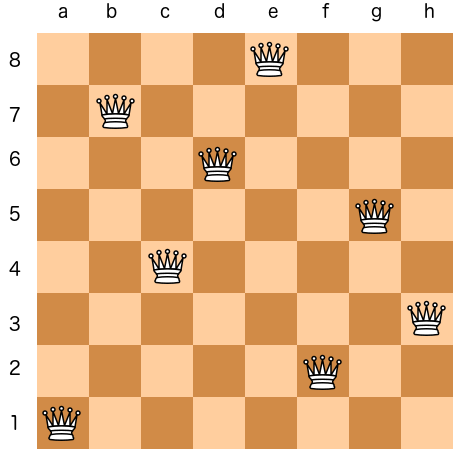
\includegraphics[width=6cm]{figs/eight_queens.png}
        \caption{A feasible solution for the 8-queens problem.}
    \end{figure}
    
    \begin{enumerate}
        \item Support we formulate the state space as the set of all arrangements of $0, 1, 2, \dots, 8$ queens on the board.
        What would each component of the search problem be?
        How many states are there?
        
        \item Give an alternative formulation which has a much smaller state space.
        List all the components of the search problem, and specify the number of states.
        % Suppose we formulate the state space as the set of all arrangements of $k = 0, 1, 2, \dots, 8$ queens in the $k$ leftmost columns with no two queens attacking each other.
        % What would each component of the search problem be?
        % How many states are there?
    \end{enumerate}

    \clearpage
    \item % Q2
    \textbf{Uniform cost graph search}.
    Consider the below state space graph.
    Perform UCS yourself and provide answers to the questions below regarding the nodes expanded during the search as well as the final path found by the algorithm.
    Remember that the search procedure should begin at node ``START", and the goal state is node ``GOAL".
    To break ties when adding nodes of equal cost to the fringe, follow the alphabetical order.
    
    Recall that UCS keeps track of the lowest cost, $c(v)$, to get from the start node to the node $v$.
    \begin{figure}[h]
        \centering
        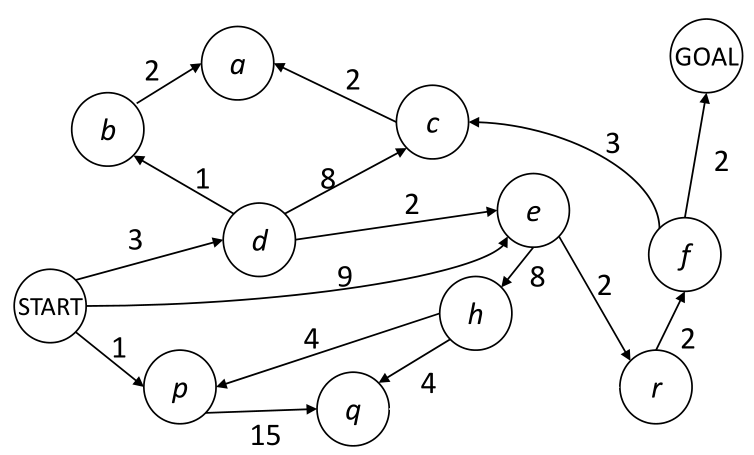
\includegraphics[width=12cm]{figs/ucs.png}
    \end{figure}
    
    % \begin{itemize}
    %     \item What is the order of nodes expanded?
    %     \item How many nodes are expanded?
    %     \item What is the final path returned?
    %     \item What is the length of path?
    %     \item What is the cost of path?
    % \end{itemize}
    \begin{enumerate}
    %     \item 
    % \end{enumerate}
        \item What is the order of nodes expanded?
        \item How many nodes are expanded?
        \item What is the final path returned?
        \item What is the length of path?
        \item What is the cost of path?
    \end{enumerate}
    
    \clearpage
    \item \textbf{The graph-coloring problem.}
    Consider a graph with n nodes that has no multiple edges and loops. We want to color the nodes in this graph. We could only use 2 colors and we need to ensure that there is no edge linking any two nodes of the same color.
    \begin{enumerate}
        \item Please judge whether the following graphs could be colored as mentioned above. Write ``Y" if you think one graph could be colored as mentioned above and write ``N" otherwise.
        
    \begin{figure}[h]
        \centering
        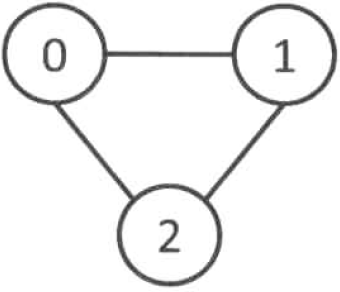
\includegraphics[width=3cm]{figs/fig2.png}
        \caption{Graph 1.}
    \end{figure}
    
    \begin{figure}[h]
        \centering
        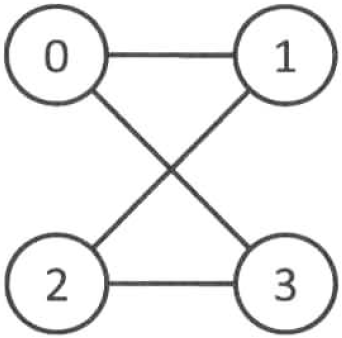
\includegraphics[width=3cm]{figs/fig3.png}
        \caption{Graph 2.}
    \end{figure}
    
    \begin{figure}[h]
        \centering
        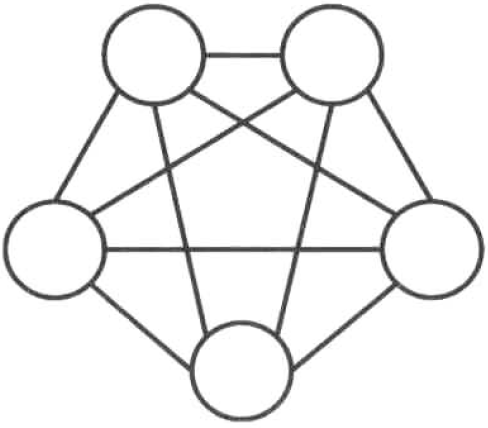
\includegraphics[width=3cm]{figs/fig4.png}
        \caption{Graph 3.}
    \end{figure}
        
        \item Please briefly describe your findings about the properties of the graphs that could be colored as mentioned above.
        
        \item We further assume the graph is \href{https://en.wikipedia.org/wiki/Connectivity_(graph_theory)}{connected}. 
        Let 1 and -1 be the two color values denoting the two colors respectively.
        Please fill in the following pseudocode for judging whether a graph could be colored as stated in the problem.  (Algorithm 2 returns ``True" if a graph could be colored as stated in the problem and returns ``False" otherwise)
\begin{algorithm}[h]
\caption{DFS}
\begin{algorithmic}[1]
\STATE\textbf{Input}: node index \textit{v}, color value \textit{c}, color list \textit{color}
\STATE \textit{color}[\textit{v}] $\gets$ \textit{c}
\FOR{\textit{neighbor} in get\_neighbor\_node(\textit{v})}
    \IF{\textit{color}[\textit{neighbor}] == \_\_\_\_}
        \RETURN False
    \ENDIF
    \IF{\textit{color}[\textit{neighbor}] == 0 and not \_\_\_\_\_\_\_\_\_\_\_\_\_\_\_\_}
        \RETURN False
    \ENDIF
\ENDFOR
\RETURN True
\end{algorithmic}
\end{algorithm}
\begin{algorithm}[h]
\caption{Color the Connected Graph}
\begin{algorithmic}[1]
\STATE\textbf{Initialize} color list \textit{color} $\gets$ $(0)^N_{i=1}$
    \IF{DFS(1,-1,\textit{color})}
        \RETURN \_\_\_\_
    % \ELSE
    %     \RETURN \_\_\_\_
    \ENDIF
\RETURN \_\_\_\_
\end{algorithmic}
\end{algorithm}

    \item 
Please modify Algorithm2 to make Algorithm2 adapt to the graph which might be not connected. (Algorithm 3 returns ``True" if a graph could be colored as stated in the problem and returns ``False" otherwise)
\begin{algorithm}[h]
\caption{Color the Graph (might be not connected)}
\begin{algorithmic}[1]
\STATE\textbf{Initialize} color list \textit{color} $\gets$ $(0)^N_{i=1}$
\FOR{\textit{node} in get\_all\_node()}
\IF{\textit{color}[\textit{node}] == 0}
    \IF{not DFS(\textit{node},-1,\textit{color})}
        \RETURN \_\_\_\_
    \ENDIF
\ENDIF
\ENDFOR
\RETURN \_\_\_\_
\end{algorithmic}
\end{algorithm}
    \end{enumerate}
    
\clearpage
\item \textbf{Explore the uniform-cost search in more depth.}
\begin{enumerate}
    \item What are the differences between the uniform-cost search and Dijkstra's algorithm? (You could click here for the reference of \href{https://en.wikipedia.org/wiki/Dijkstra%27s_algorithm}{Dijkstra's algorithm}.)
    \item If there are some arcs with negative costs in the graph, does the uniform-cost search still work? Give a concrete example to support your argument.
    \item Introduce one  algorithm which you know and is able to find the least-cost path in the graph containing the arcs with negative costs.
\end{enumerate}
\end{enumerate}

\end{document} 